         \chapter{Chemical bonding}\fancyfoot[LO,RE]{Chemistry: Matter and Materials}
    \setcounter{figure}{1}
    \setcounter{subfigure}{1}
    \label{m38704*cid1}
            \section{Introduction}
            \nopagebreak
%            \label{m38704} $ \hspace{-5pt}\begin{array}{cccccccccccc}   
\includegraphics[width=0.75cm]{col11305.imgs/summary_fullmarks.png} &   \end{array} $ \hspace{2 pt}\raisebox{-5 pt}{} {(section shortcode: P10030 )} \par 
      \label{m38704*id138190}When you look at everything around you and what it is made of, you will realise that atoms seldom exist on their own. More often, the things around us are made up of different atoms that have been joined together. This is called \textbf{chemical bonding}. Chemical bonding is one of the most important processes in chemistry because it allows all sorts of different molecules and combinations of atoms to form, which then make up the objects in the complex world around us.\par 
    \label{m38704*cid4}
            \subsection*{What happens when atoms bond?}
            \nopagebreak
      \label{m38704*id138842}A \textbf{chemical bond} is formed when atoms are held together by attractive forces. This attraction occurs when electrons are \textsl{shared} between atoms, or when electrons are \textsl{exchanged} between the atoms that are involved in the bond. The sharing or exchange of electrons takes place so that the outer energy levels of the atoms involved are filled, making the atoms are more stable. If an electron is \textbf{shared}, it means that it will spend its time moving in the electron orbitals around \textsl{both} atoms. If an electron is \textbf{exchanged} it means that it is transferred from one atom to another. In other words one atom \textsl{gains} an electron while the other \textsl{loses} an electron.\par 
\label{m38704*fhsst!!!underscore!!!id83}
\Definition{Chemical bond} {A chemical bond is the physical process that causes atoms and molecules to be attracted to each other and held together in more stable chemical compounds.} 
      \label{m38704*id138909}The type of bond that is formed depends on the elements that are involved. In this chapter, we will be looking at three types of chemical bonding: \textbf{covalent}, \textbf{ionic} and \textbf{metallic bonding}.\\
      \label{m38704*id138929}You need to remember that it is the \textsl{valence electrons} (those in the outermost level) that are involved in bonding and that atoms will try to fill their outer energy levels so that they are more stable. The noble gases have completely full outer energy levels, so are very stable and do not react easily with other atoms.\\
         \section{Lewis structures}
    \nopagebreak
%            \label{m38701} $ \hspace{-5pt}\begin{array}{cccccccccccc}   
\includegraphics[width=0.75cm]{col11305.imgs/summary_fullmarks.png} &   \end{array} $ \hspace{2 pt}\raisebox{-5 pt}{} {(section shortcode: P10031 )} \par 
      \label{m38701*id140105}\textbf{Lewis notation} uses dots and crosses to represent the \textbf{valence electrons} on different atoms. The chemical symbol of the element is used to represent the nucleus and the inner electrons of the atom. To determine which are the valence electrons we look at the last \textsl{energy level} in the atom's electronic structure (chapter~\ref{chap:atom}). For example, silicon's electronic structure can be written as:$1\text{s}^{2}2\text{s}^{2}2\text{p}^{6}3\text{s}^{2}3\text{p}^{2}$ or $\text{[Ne]}3\text{s}^{2}3\text{p}^{2}$. The last energy level is the 3rd one and it contains 4 electrons. These are the valence electrons.
\Tip{If we write the condensed electron configuration, then we can easily see the valence electrons.}
 \par 
So, for example, a hydrogen atom would be represented like this: 
% \begin{center}
\scalebox{0.8}{
\begin{pspicture}(1.5,1.5)(2.5,2.1)
%\psgrid[gridcolor=lightgray]
\rput(2,2){\Large \textbf{$\text{H}$}}
\rput(2.5,2){$\bullet$}
\end{pspicture}
}
% \end{center}

A chlorine atom would look like this:
% \begin{center}
\scalebox{0.8}{
\begin{pspicture}(-1,-0.6)(2,0.4)
%\psgrid[gridcolor=lightgray]
\rput(1,0){\Large \textbf{$\text{Cl}$}}
\uput{9pt}[d](1,0){$\times$ $\times$}
\rput{90}(1,0){\uput{9pt}[d](0,0){$\times$ $\times$}}
\rput{180}(1,0){\uput{9pt}[d](0,0){$\times$ $\times$}}
\rput{270}(1,0){\uput{9pt}[d](0,0){$\times$}}
\end{pspicture}
}
% \end{center}

A molecule of hydrogen chloride would be shown like this:
\begin{center}
\scalebox{0.8}{
\begin{pspicture}(-1,-0.6)(2,0.6)
%\psgrid[gridcolor=lightgray]
\rput(1,0){\Large \textbf{$\text{Cl}$}}
\uput{9pt}[d](1,0){$\times$ $\times$}
\rput{90}(1,0){\uput{9pt}[d](0,0){$\times$ $\times$}}
\rput{180}(1,0){\uput{9pt}[d](0,0){$\times$ $\times$}}
\rput{270}(1,0){\uput{9pt}[d](0,0){$\times$ $\bullet$}}
\rput(0,0){\Large \textbf{$\text{H}$}}
\end{pspicture}
}
\end{center}

      \par 
      \label{m38701*id140178}The dot and cross in between the two atoms, represent the pair of electrons that are shared in the covalent bond.\par 
Table~\ref{tab:lewis} gives some further examples of Lewis diagrams.
\begin{table}[H]
 \begin{center}
  \begin{tabular}{|l|l|l|} \hline
   Iodine & $\text{I}_2$ & 
\begin{pspicture}(-2,-0.4)(4,0.4)
%\psgrid[gridcolor=gray]
\rput(1,0){\Large \textbf{$\text{I}$}}
\uput{9pt}[d](1,0){$\times$ $\times$}
\rput{180}(1,0){\uput{9pt}[d](0,0){$\times$ $\times$}}
\rput{270}(1,0){\uput{9pt}[d](0,0){$\times$ $\times$}}
\rput(2,0){\Large \textbf{$\text{I}$}}
\uput{9pt}[d](2,0){$\bullet$ $\bullet$}
\rput{90}(2,0){\uput{9pt}[d](0,0){$\bullet$ $\bullet$}}
\rput{180}(2,0){\uput{9pt}[d](0,0){$\bullet$ $\bullet$}}
\rput{270}(2,0){\uput{9pt}[d](0,0){$\times$ $\bullet$}}
\end{pspicture} \\ \hline
   Water & $\text{H}_{2}\text{O}$ & 
\begin{pspicture}(-0.2,-0.4)(2,0.4)
%\psgrid[gridcolor=gray]
\rput(0.1,0){\Large \textbf{$\text{H}$}}
\rput(1,0){\Large \textbf{$\text{O}$}}
\uput{9pt}[d](1,0){$\times$ $\bullet$}
\rput{90}(1,0){\uput{9pt}[d](0,0){$\times$ $\times$}}
\rput{180}(1,0){\uput{9pt}[d](0,0){$\times$ $\times$}}
\rput{270}(1,0){\uput{9pt}[d](0,0){$\times$ $\bullet$}}
\rput(1,-0.8){\Large \textbf{$\text{H}$}}
\end{pspicture} \\ \hline
   Carbon dioxide & $\text{CO}_2$ &
\begin{pspicture}(-2,-0.4)(4,0.4)
%\psgrid[gridcolor=gray]
\rput(0.1,0){\Large \textbf{$\text{O}$}}
\rput{220}(.1,0){\uput{9pt}[d](0,0){$\bullet$ $\bullet$}}
\rput{320}(.1,0){\uput{9pt}[d](0,0){$\bullet$ $\bullet$}}
\rput{90}(0,0){\uput{9pt}[d](0,0){$\bullet$ $\bullet$ }}
\rput(1,0){\Large \textbf{$\text{C}$}}
\rput{270}(1,0){\uput{9pt}[d](0,0){$\times$ $\times$}}
\rput{90}(1,0){\uput{9pt}[d](0,0){$\times$ $\times$ }}
\rput(2,0){\Large \textbf{$\text{O}$}}
\rput{40}(2,0){\uput{9pt}[d](0,0){$\bullet$ $\bullet$}}
\rput{140}(2,0){\uput{9pt}[d](0,0){$\bullet$ $\bullet$}}
\rput{270}(2,0){\uput{9pt}[d](0,0){$\bullet$ $\bullet$ }}
\end{pspicture} \\ \hline
   Hydrogen cyanide & $\text{HCN}$ &
\begin{pspicture}(-2,-0.4)(4,0.4)
%\psgrid[gridcolor=gray]
\rput(0.1,0){\Large \textbf{$\text{H}$}}
\rput(1,0){\Large \textbf{$\text{C}$}}
\rput{270}(1,0){\uput{9pt}[d](0,0){$\times$ $\bullet$}}
\rput{90}(1,0){\uput{9pt}[d](0,0){$\times$ $\times$ $\times$}}
\rput(2,0){\Large \textbf{$\text{N}$}}
\rput{90}(2,0){\uput{9pt}[d](0,0){$\bullet$ $\bullet$}}
\rput{270}(2,0){\uput{9pt}[d](0,0){$\bullet$ $\bullet$ $\bullet$}}
\end{pspicture} \\ \hline  
  \end{tabular}
\caption{Lewis diagrams for some simple molecules}
\label{tab:lewis}
 \end{center}
\end{table}
For carbon dioxide, you can see how we represent a double bond in Lewis notation. As there are two bonds between each oxygen atom and the carbon atom, two pairs of valence electrons link them. Similarly, hydrogen cyanide shows how to represent a triple bond.
    \noindent
\label{m38701*secfhsst!!!underscore!!!id327}
            \begin{exercises}{Lewis structures}
            \nopagebreak \noindent
      \label{m38701*id140889}\begin{enumerate}[noitemsep, label=\textbf{\arabic*}. ] 
%Question 1
            \label{m38701*uid23}\item Represent each of the following \textsl{atoms} using Lewis notation:
\label{m38701*id140910}\begin{enumerate}[noitemsep, label=\textbf{\alph*}. ] 
            \label{m38701*uid24}\item beryllium
\label{m38701*uid25}\item calcium
\label{m38701*uid26}\item lithium
\end{enumerate}
%Question 2
                \label{m38701*uid27}\item Represent each of the following \textsl{molecules} using Lewis notation:
\label{m38701*id140969}\begin{enumerate}[noitemsep, label=\textbf{\alph*}. ] 
            \label{m38701*uid28}\item bromine gas ($\text{Br}{}_{2}$)
\label{m38701*uid29}\item carbon dioxide ($\text{CO}{}_{2}$)
\end{enumerate}
%Question 3 (2 on FM)
Which of these two molecules contains a double bond?\newline
%Question 4
\label{m38701*uid31}\item Two chemical reactions are described below.
\label{m38701*id141048}\begin{itemize}[noitemsep]
            \label{m38701*uid32}\item nitrogen and hydrogen react to form $\text{NH}_{3}$\label{m38701*uid33}
\item carbon and hydrogen bond to form a molecule of $\text{CH}_{4}$\end{itemize}
For each reaction, give:
\label{m38701*id141106}\begin{enumerate}[noitemsep, label=\textbf{\alph*}. ] 
\item the number of electrons in the outermost energy level
\label{m38701*uid35}\item the Lewis structure of the product that is formed
\label{m38701*uid36}\item the chemical formula of the product
\label{m38701*uid37}\item the name of the product
\end{enumerate}
%Question 5
                \label{m38701*uid38}\item A chemical compound has the following Lewis notation:
    \setcounter{subfigure}{0}
	\begin{figure}[H] % horizontal\label{m38701*id141174}
\begin{center}
\scalebox{.8}{
\begin{pspicture}(1,-1)(2,0.4)
%\psgrid[gridcolor=gray]
\rput(0.1,0){\Large \textbf{X}}
\rput(1,0){\Large \textbf{Y}}
\uput{9pt}[d](1,0){$\times$ $\bullet$}
\rput{90}(1,0){\uput{9pt}[d](0,0){$\times$ $\times$}}
\rput{180}(1,0){\uput{9pt}[d](0,0){$\times$ $\times$}}
\rput{270}(1,0){\uput{9pt}[d](0,0){$\times$ $\bullet$}}
\rput(1,-0.8){\Large \textbf{H}}
\end{pspicture}
}
\end{center}
 \end{figure}       \label{m38701*id141181}\begin{enumerate}[noitemsep, label=\textbf{\alph*}. ] 
            \label{m38701*uid39}\item How many valence electrons does element $\text{Y}$ have?
\label{m38701*uid40}\item What is the valency of element $\text{Y}$? (remember that the valency of an atom is the number of chemical bonds it can form.)
\label{m38701*uid41}\item What is the valency of element $\text{X}$?
\label{m38701*uid42}\item How many covalent bonds are in the molecule?
\label{m38701*uid43}\item Suggest a name for the elements $\text{X}$ and $\text{Y}$.
\end{enumerate}
                \end{enumerate}
  \label{m38701**end}
\par \raisebox{-5 pt}{
\includegraphics[width=0.5cm]{col11305.imgs/summary_www.png}} Find the answers with the shortcodes:
 \par \begin{tabular}[h]{cccccc}
 (1.) lOC  &  (2.) lOa  &  (3.) lj2  &  (4.) lOx  &  (5.) lOc  & \end{tabular}
\end{exercises}
    \label{m38704*cid5}
            \section{Covalent Bonding}
            \nopagebreak
            \label{m38704*uid6}
            \subsection*{The nature of the covalent bond}
            \nopagebreak
        \label{m38704*id138956}Covalent bonding occurs between the atoms of \textbf{non-metals}. The outermost orbitals of the atoms overlap so that unpaired electrons in each of the bonding atoms can be shared. By overlapping orbitals, the outer energy shells of all the bonding atoms are filled. The shared electrons move in the orbitals around \textsl{both} atoms. As they move, there is an attraction between these negatively charged electrons and the positively charged nuclei. This attractive force holds the atoms together in a covalent bond.\par 
\label{m38704*fhsst!!!underscore!!!id94}
\Definition{ \label{id2427171} Covalent bond} { \label{m38704*meaningfhsst!!!underscore!!!id94}
Covalent bonding is a form of chemical bonding where pairs of electrons are shared between atoms.} 
\label{m38704*id139505}You will have noticed in table~\ref{tab:lewis} that the number of electrons that are involved in bonding varies between atoms.
\Tip{There is a relationship between the valency of an element and its position on the periodic table. For the elements in groups 1 and 2, the valency is the group number. For the elements in groups 13 - 18, the valency is the group number minus $10$. For the transition metals, the valency can vary. In these cases we indicate the valency by a roman numeral after the element name, e.g. iron (III) chloride.}
 We can say the following:
\begin{itemize}
 \item A \textbf{single covalent} bond is formed when two electrons are shared between the same two atoms, one electron from each atom. 
 \item A \textbf{double covalent} bond is formed when four electrons are shared between the same two atoms, two electrons from each atom.
 \item A \textbf{triple covalent} bond is formed when six electrons are shared between the same two atoms, three electrons from each atom.
\end{itemize}
You should also have noticed that compounds can have a mixture of single, double and triple bonds and that an atom can have several bonds. In other words, an atom does not need to share all its valence electrons with one other atom, but can share its valence electrons with several different atoms.\\
We say that the \textbf{valency} of the atoms is different. 
\Definition{Valency}{The number of electrons in the outer shell of an atom which are able to be used to form bonds with other atoms.}

\label{m38704*id138991}Below are a few examples. Remember that it is only the \textsl{valence electrons} that are involved in bonding and so when diagrams are drawn to show what is happening during bonding, it is only these electrons that are shown. \par 
\label{m38704*secfhsst!!!underscore!!!id98} 
\begin{wex}{Covalent bonding}{How do hydrogen and chlorine atoms bond covalently in a molecule of hydrogen chloride?}{\westep{Determine the electron configuration of each of the bonding atoms.}
A chlorine atom has 17 electrons and an electron configuration of $\text{[Ne]}3\text{s}^{2}3\text{p}^{5}$. A hydrogen atom has only 1 electron and an electron configuration of $1\text{s}^{1}$.
\westep{Determine how many of the electrons are paired or unpaired.}
Chlorine has 7 valence electrons. One of these electrons is unpaired. Hydrogen has 1 valence electron and it is unpaired.
\westep{Work out how the electrons are shared}
The hydrogen atom needs one more electron to complete its outermost energy level. The chlorine atom also needs one more electron to complete its outermost energy level. Therefore \textit{one pair of electrons} must be shared between the two atoms. A single covalent bond will be formed.
\begin{figure}[H]
\begin{center}
\scalebox{0.6}{
\begin{pspicture}(-7,-4.5)(7,1.5)
%\psgrid
\rput(-3.5,-1.8){\textbf{+}}
% Lower left
\uput[u](-5,-2){
\pscircle(0,0){1}
\qdisk(0.83,0.45){0.2}
\pscircle(3.5,0){1.5}
\uput{0}[u](0,-.2){\scalebox{2}{$\text{H}$}}

\rput(1.25,0){ 
\uput[d](0.83,-0.1){ \scalebox{2}{x}}
\uput{0.01}[l](2.25,1.5){ \scalebox{2}{x}}
\uput{0.01}[r](2.25,1.5){ \scalebox{2}{x}}
\uput[u](3.65,0){ \scalebox{2}{x}}
\uput[d](3.65,0){ \scalebox{2}{x}}
\uput{0.01}[l](2.25,-1.45){ \scalebox{2}{x}}
\uput{0.01}[r](2.25,-1.45){ \scalebox{2}{x}} 
\uput{0}[u](2.25,-.2){\scalebox{2}{$\text{Cl}$}}
}
}

% \psline{->}(0.5,2)(1.5,2)
\psline{->}(0.65,-2)(1.65,-2)

% Lower right
\uput[u](3,-2){
\pscircle(0,0){1}
\pscircle(2.25,0){1.5}
\qdisk(0.83,0.45){0.2}
\uput{0}[u](0,-.2){\scalebox{2}{$\text{H}$}}

\uput[d](0.83,-0.1){ \scalebox{2}{x}}
\uput{0.01}[l](2.25,1.5){ \scalebox{2}{x}}
\uput{0.01}[r](2.25,1.5){ \scalebox{2}{x}}
\uput[u](3.65,0){ \scalebox{2}{x}}
\uput[d](3.65,0){ \scalebox{2}{x}}
\uput{0.01}[l](2.25,-1.45){ \scalebox{2}{x}}
\uput{0.01}[r](2.25,-1.45){ \scalebox{2}{x}} 
\uput{0}[u](2.25,-.2){\scalebox{2}{$\text{Cl}$}}
}
\end{pspicture}
}
\end{center}
% \caption{Covalent bonding in a molecule of hydrogen chloride}
\label{fig:bonding:hydrogen chloride}
\end{figure}
}
\end{wex}
    \noindent
\par 
\begin{wex}{Covalent bonding involving multiple bonds }{
 %problem
        \label{m38704*id139185}How do nitrogen and hydrogen atoms bond to form a molecule of ammonia ($\text{NH}{}_{3}$)? 
      
}
{
%solution
\westep{Give the electron configuration} 
        \label{m38704*id139225}A nitrogen atom has seven electrons, and an electron configuration of $\text{[He]}2\text{s}^{2}2\text{p}^{3}$. A hydrogen atom has only 1 electron, and an electron configuration of $1\text{s}^{1}$.
        \westep{Give the number of valence electrons}  
        \label{m38704*id139283}Nitrogen has five valence electrons. Three of these electrons are unpaired. Hydrogen has one valence electron and it is unpaired. 
        \westep{Work out how the electrons are shared} 
        \label{m38704*id139292}Each hydrogen atom needs one more electron to complete its valence energy shell. The nitrogen atom needs three more electrons to complete its valence energy shell. Therefore \textsl{three pairs of electrons} must be shared between the four atoms involved. Three single covalent bonds will be formed. 
    \setcounter{subfigure}{0}
\begin{figure}[H]
\scalebox{0.6}{
\begin{pspicture}(-9,1)(9,7)
%\psgrid
\rput(-3.5,4.2){\textbf{+}}
% Upper left
\uput[u](-5,4){
\rput(-1.75,0.25){\scalebox{ 2}{ {\bf 3} }}
\pscircle(-0.25,0){1}
\qdisk(0.58,0.45){0.2}
\uput{0}[u](-0.25,-.2){\scalebox{2}{$\text{H}$}}

\rput(1.25,0){ 
\pscircle(2.25,0){1.5}
\uput[d](0.83,-0.1){ \scalebox{2}{x}} % left side

\uput{0.01}[l](2.25,1.5){ \scalebox{2}{x}} % top
\uput{0.01}[r](2.25,1.5){ \scalebox{2}{x}}

\uput[u](3.65,0){ \scalebox{2}{x}} % right side
\uput{0.01}[l](2.25,-1.45){ \scalebox{2}{x}} % bottom
\uput{0}[u](2.25,-.2){\scalebox{2}{$\text{N}$}} % N label
}
}

\psline{->}(0.5,4)(1.5,4)

% Upper right
\uput[u](3,4){
\rput(-0.25,0){ 
\pscircle(2.25,0){1.5}
\uput[d](0.83,-0.1){ \scalebox{2}{x}} % left side

\uput{0.01}[l](2.25,1.5){ \scalebox{2}{x}} % top
\uput{0.01}[r](2.25,1.5){ \scalebox{2}{x}}

\uput{0.3}[u](3.65,0){ \scalebox{2}{x}} % right side
\uput{0.1}[r](2.25,-1.4){ \scalebox{2}{x}} % bottom
\uput{0}[u](2.25,-.2){\scalebox{2}{$\text{N}$}} % N label
}
\rput(0,0){
\pscircle(-0.25,0){1}
\qdisk(0.58,0.45){0.2}
\uput{0}[u](-0.25,-.2){\scalebox{2}{$\text{H}$}}
} 
\rput(4.5,0){
\pscircle(-0.25,0){1}
\qdisk(-1.1,-0.45){0.2}
\uput{0}[u](-0.25,-.2){\scalebox{2}{$\text{H}$}}
} 
\rput(2.25,-2.25){
\pscircle(-0.25,0){1}
\qdisk(-0.75,0.9){0.2}
\uput{0}[u](-0.25,-.2){\scalebox{2}{$\text{H}$}}
} 
}
\end{pspicture}
}
\end{figure}
 
}
\end{wex}
    \noindent 
\begin{wex}{Covalent bonding involving a double bond}{How do oxygen atoms bond covalently to form an oxygen molecule?\\}
{
\westep{Determine the electron configuration of the bonding atoms.}
Each oxygen atom has 8 electrons, and their electron configuration is $\text{[He]}2\text{s}^{2}2\text{p}^{4}$. 

\westep{Determine the number of valence electrons for each atom and how many of these electrons are paired and unpaired.}
Each oxygen atom has 6 valence electrons. Each atom has 2 unpaired electrons.

\westep{Work out how the electrons are shared}

Each oxygen atom needs two more electrons to complete its valence energy shell. Therefore \textit{two pairs of electrons} must be shared between the two oxygen atoms so that both outermost energy levels are full. A double bond is formed.

\begin{figure}[H]
\scalebox{0.7}{
\begin{pspicture}(-9,-4)(9,1)
 %\psgrid
\rput(-3.4,-1.8){\textbf{+}}
% Lower left
\uput[u](-5,-2){
\rput(-2.5,0){ 
\pscircle(2.25,0){1.5}
\uput[u](0.83,-0.1){ \scalebox{2}{x}} % left side
\uput[d](0.83,-0.1){ \scalebox{2}{x}} % left side

\uput{0.01}[l](2.25,1.5){ \scalebox{2}{x}} % top
\uput{0.01}[r](2.25,1.5){ \scalebox{2}{x}}

\uput[u](3.65,0){ \scalebox{2}{x}} % right side
\uput{0.01}[l](2.25,-1.45){ \scalebox{2}{x}} % bottom
\uput{0}[u](2.25,-.2){\scalebox{2}{$\text{O}$}} % O label
}
\rput(1.25,0){ 
\pscircle(2.25,0){1.5}
\uput[d](0.83,-0.1){ \qdisk(0,0){0.2} } % left side

\uput{0.3}[l](2.25,1.5){ \qdisk(0,0){0.2}} % top
\uput{0.3}[r](2.25,1.5){ \qdisk(0,0){0.2}}

\uput{0.3}[u](3.65,0){ \qdisk(0,0){0.2}} % right side
\uput{0.3}[d](3.65,0){ \qdisk(0,0){0.2}} % right side
\uput{0.3}[l](2.25,-1.45){ \qdisk(0,0){0.2}} % bottom
\uput{0}[u](2.25,-.2){\scalebox{2}{$\text{O}$}} % O label
}
}


\psline{->}(0.65,-2)(1.65,-2)


% Lower right
\uput[u](3,-2){
\rput(-1.5,0){ 
\pscircle(2.25,0){1.5}
\uput[u](0.83,-0.1){ \scalebox{2}{x}} % left side
\uput[d](0.83,-0.1){ \scalebox{2}{x}} % left side

\uput{0.01}[l](2.25,1.5){ \scalebox{2}{x}} % top
\uput{0.01}[r](2.25,1.5){ \scalebox{2}{x}}

\uput[u](3.4,0){ \scalebox{2}{x}} % right side
\uput[d](3.4,0){ \scalebox{2}{x}} % right side
\uput{0}[u](2.25,-.2){\scalebox{2}{$\text{O}$}} % O label
}
\rput(1.25,0){ 
\pscircle(2.25,0){1.5}
\uput{0.35}[u](1.06,-0.02){ \qdisk(0,0){0.2} } % left side
\uput{0.35}[d](1.06,-0.02){ \qdisk(0,0){0.2} } % left side

\uput{0.3}[l](2.25,1.5){ \qdisk(0,0){0.2}} % top
\uput{0.3}[r](2.25,1.5){ \qdisk(0,0){0.2}}

\uput{0.3}[u](3.65,0){ \qdisk(0,0){0.2}} % right side
\uput{0.3}[d](3.65,0){ \qdisk(0,0){0.2}} % right side
\uput{0}[u](2.25,-.2){\scalebox{2}{$\text{O}$}} % O label
}
}

\end{pspicture}
}
\end{figure}
}
\end{wex}
            \subsection*{Properties of covalent compounds}
            \nopagebreak
            \label{m38704*eip-541}
Covalent compounds have several properties that distinguish them from ionic compounds and metals. These properties are:
\label{m38704*di6325}\begin{enumerate}[noitemsep, label=\textbf{\arabic*}. ] 
            \item The melting and boiling points of covalent compounds are generally lower than those of ionic compounds.
\item Covalent compounds are generally more flexible than ionic compounds. The molecules in covalent compounds are able to move around to some extent and can sometimes slide over each other (as is the case with graphite, which is why the lead in your pencil feels slightly slippery). In ionic compounds, all the ions are tightly held in place.
\item Covalent compounds generally are not very soluble in water, for example plastics are covalent compounds and many plastics are water resistant.
\item Covalent compounds generally do not conduct electricity when dissolved in water, for example iodine dissolved in pure water does not conduct electricity.\end{enumerate}
\par 
    \noindent 
\label{m38704*secfhsst!!!underscore!!!id172}
            \begin{exercises}{Covalent bonding
        }
            \nopagebreak \noindent
        \label{m38704*id139588}\begin{enumerate}[noitemsep, label=\textbf{\arabic*}. ] 
%Question 1
            \label{m38704*uid10}\item Explain the difference between the \textsl{valence electrons} and the \textsl{valency} of an element.\newline
%Question 2
\label{m38704*uid11}\item Complete the table below by filling in the number of valence electrons for each of the elements shown:
    % \textbf{m38704*id139625}\par
          \begin{table}[H]
    % \begin{table}[H]
    % \\ 'id2897338' '1'
        \begin{center}
      \label{m38704*id139625}
    \noindent
      \begin{tabular}{|l|l|p{3cm}|p{3cm}|}\hline
\textbf{Element} & \textbf{Group number} & \textbf{No. of valence electrons} & \textbf{No. of electrons needed to fill outer shell}  \\ \hline
        $\text{He}$ & & & \\ \hline
        $\text{Li}$ & & & \\ \hline
        $\text{B}$ & & & \\ \hline
        $\text{C}$ & & & \\ \hline
        $\text{F}$ & & & \\ \hline
        $\text{Ne}$ & & & \\ \hline
        $\text{Na}$ & & & \\ \hline
        $\text{Al}$ & & & \\ \hline
        $\text{P}$ & & & \\ \hline
        $\text{S}$ & & & \\ \hline
        $\text{Ca}$ & & & \\ \hline
        $\text{Kr}$ & & & \\ \hline
    \end{tabular}
      \end{center}
\end{table}
    \par
%Question 3
          \label{m38704*uid12}\item Draw simple diagrams to show how electrons are arranged in the following covalent molecules:
\label{m38704*id140030}\begin{enumerate}[noitemsep, label=\textbf{\alph*}. ] 
            \label{m38704*uid13}\item hydrogen sulphide ($\text{H}_{2}\text{S}$)
\label{m38704*uid14}\item chlorine ($\text{Cl}_{2}$)
\item nitrogen ($\text{N}_2$)
\item carbon monoxide ($\text{CO}$)
\end{enumerate}
                \end{enumerate}
      \label{m38704*eip-790}
\par \raisebox{-5 pt}{
\includegraphics[width=0.5cm]{col11305.imgs/summary_www.png}} Find the answers with the shortcodes:
 \par \begin{tabular}[h]{cccccc}
 (1.) lOY  &  (2.) ljT  &  (3.) ljb  & \end{tabular}
\end{exercises}

         \section{Ionic bonding}
    \nopagebreak
%            \label{m38684} $ \hspace{-5pt}\begin{array}{cccccccccccc}   \end{array} $ \hspace{2 pt}\raisebox{-5 pt}{
\includegraphics[width=0.5cm]{col11305.imgs/summary_www.png}} {(section shortcode: P10032 )} \par 
      \label{m38684*uid54}
            \subsection*{The nature of the ionic bond}
            \nopagebreak
        \label{m38684*id142190}When electrons are \textsl{transferred} from one atom to another it is called \textbf{ionic bonding}.\par 
        \label{m38684*id142218}Electronegativity is a property of an atom, describing how strongly it attracts or holds onto electrons. Ionic bonding takes place when the difference in electronegativity between the two atoms is more than $1.7$. This usually happens when a metal atom bonds with a non-metal atom. When the difference in electronegativity is large, one atom will attract the shared electron pair much more strongly than the other, causing electrons to be transferred to the atom with higher electronegativity. When ionic bonds form, a metal donates one or more electrons, due to having a low electronegativity, to form a positive ion or cation. The non-metal atom has a high electronegativity, and therefore readily gains electrons to form a negative ion or anion. The two ions are then attracted to each other by electrostatic forces. \par 
\label{m38684*fhsst!!!underscore!!!id456}
\Definition{   \label{id2430088} Ionic bond } { \label{m38684*meaningfhsst!!!underscore!!!id456}
        An ionic bond is a type of chemical bond where one or more electrons are transferred from one atom to another.
         } 
        \label{m38684*id142248}
          \textbf{Example 1:}
        \par 
        \label{m38684*id142255}In the case of $\text{NaCl}$, the difference in electronegativity between $\text{Na}$ (0,93) and $\text{Cl}$ (3,16) is $2,1$. Sodium has only one valence electron, while chlorine has seven. Because the electronegativity of chlorine is higher than the electronegativity of sodium, chlorine will attract the valence electron of the sodium atom very strongly. This electron from sodium is transferred to chlorine. Sodium loses an electron and forms an ${\text{Na}}^{+}$ ion. \\
 \scalebox{0.8}{
\begin{pspicture}(1.5,1.5)(2.5,2.1)
%\psgrid[gridcolor=lightgray]
\rput(2,2){\Large \textbf{$\text{Na}$}}
\rput(2.5,2){$\bullet$}
\psline[arrowsize=0.2]{->}(2.75,1.95)(3.75,1.95)
\rput(4.8,2.1){\Large \textbf{$+$}}
\rput(4.4,2){\Large \textbf{$\text{Na}$}}
\rput(5.5,2){\Large{$+$}}
\rput(6.6,2){\Large{electron}}
\end{pspicture}
} \par
Chlorine gains an electron and forms an ${\text{Cl}}^{-}$ ion. \\
 \scalebox{0.8}{
\begin{pspicture}(1.5,1.5)(2.5,2.1)
%\psgrid[gridcolor=lightgray]
\rput(2,2){\Large \textbf{$\text{Cl}$}}
\uput{9pt}[d](2,2){$\times$ $\times$}
\rput{90}(2,2){\uput{9pt}[d](0,0){$\times$ $\times$}}
\rput{180}(2,2){\uput{9pt}[d](0,0){$\times$ $\times$}}
\rput{270}(2,2){\uput{9pt}[d](0,0){$\times$}}
\rput(3.2,2){\Large{$+$}}
\rput(4.6,2){\Large{electron}}
\psline[arrowsize=0.2]{->}(5.75,1.95)(6.75,1.95)
\rput(7.85,2){\scalebox{2}{[\hspace{0.04cm}$\text{Cl}$ \hspace{0.04cm}]$^-$}} 
		\rput(7.6,2){
			\uput{0.05}[l](0,0.5){$\times$}		% Top
			\uput{0.05}[r](0,0.5){$\times$}
			\uput{0.05}[u](0.5,0){$\times$}		% Right
			\uput{0.05}[d](0.5,0){$\times$}
			\uput{0.05}[l](0,-0.5){$\times$}		% Bottom
			\uput{0.05}[r](0,-0.5){$\times$}	
			\uput{0.05}[u](-0.5,0){$\times$}		% Left			
			\uput{0.05}[d](-0.5,0){$\bullet$}
		}
\end{pspicture}
} \par
\Note{Chlorine is a diatomic molecule and so for it to take part in ionic bonding, it must first break up into two atoms of chlorine. Sodium is part of a metallic lattice and the individual atoms must first break away from the lattice.}
        \label{m38684*id142337}The electron is therefore transferred from sodium to the chloride ion:\par 
    \setcounter{subfigure}{0}
\begin{figure}[!h]
\begin{center}
\begin{pspicture}(-3,-1.4)(6,1)
\rput(-2.6,0.1){\Large \textbf{$+$}}
\rput(-3,0){\Large \textbf{$\text{Na}$}}
\rput(-2,0){\Large{$+$}}
\rput(-0.68,0){\scalebox{2}{[\hspace{0.04cm}$\text{Cl}$ \hspace{0.04cm}]$^-$}} 
		\rput(-0.9,0){
			\uput{0.05}[l](0,0.5){$\times$}		% Top
			\uput{0.05}[r](0,0.5){$\times$}
			\uput{0.05}[u](0.5,0){$\times$}		% Right
			\uput{0.05}[d](0.5,0){$\times$}
			\uput{0.05}[l](0,-0.5){$\times$}		% Bottom
			\uput{0.05}[r](0,-0.5){$\times$}	
			\uput{0.05}[u](-0.5,0){$\times$}		% Left			
			\uput{0.05}[d](-0.5,0){$\bullet$}
		}
\psline[arrowsize=0.2]{->}(0.75,0)(1.75,0)
\rput(4.05,0){ \scalebox{2}{$\text{[Na]}^+ $[\hspace{0.02cm}  $\text{Cl}$ \hspace{0.02cm}]$^-$} }
\rput(4.7,0){
  \uput{0.05}[l](0,0.5){$\times$}		% Top
  \uput{0.05}[r](0,0.5){$\times$}
  \uput{0.05}[u](0.5,0){$\times$}		% Right
  \uput{0.05}[d](0.5,0){$\times$}
  \uput{0.05}[l](0,-0.5){$\times$}		% Bottom
  \uput{0.05}[r](0,-0.5){$\times$}	
  \uput{0.05}[u](-0.5,0){$\times$}		% Left			
  \uput{0.05}[d](-0.5,0){$\bullet$}
}

\end{pspicture}
	
\caption{Ionic bonding in sodium chloride}
\end{center}
\end{figure}   
        \label{m38684*id142300}The balanced equation for the reaction is:\par 
        \label{m38684*id142305}\nopagebreak\noindent{}
    \begin{equation*}
    2\text{Na}+\text{Cl}_{2}\to 2\text{NaCl}
      \end{equation*}    

        \label{m38684*id142353}
          \textbf{Example 2:}
        \par 
        \label{m38684*id142360}Another example of ionic bonding takes place between magnesium ($\text{Mg}$) and oxygen ($\text{O}_2$) to form magnesium oxide ($\text{MgO}$). Magnesium has two valence electrons and an electronegativity of 1,31, while oxygen has six valence electrons and an electronegativity of 3,44. Since oxygen has a higher electronegativity, it attracts the two valence electrons from the magnesium atom and these electrons are transferred from the magnesium atom to the oxygen atom. Magnesium loses two electrons to form ${\text{Mg}}^{2+}$, and oxygen gains two electrons to form ${\text{O}}^{2-}$. The attractive force between the oppositely charged ions is what holds the compound together.\par 
        \label{m38684*id138529}The balanced equation for the reaction is:\par 
        \label{m38684*id138535}\nopagebreak\noindent{}
    \begin{equation*}
    2\text{Mg}+{\text{O}}_{2}\to 2\text{MgO}
      \end{equation*}
        \label{m38684*id142521}Because oxygen is a diatomic molecule, two magnesium atoms will be needed to combine with one oxygen molecule (which has two oxygen atoms) to produce two units of magnesium oxide ($\text{MgO}$).\par 
%     \setcounter{subfigure}{0}
% \begin{figure}[!h]
% \begin{center}
% \begin{pspicture}(-3,-1.2)(6,1)
% 		%\psgrid
% 		\psline[linearc=0.25]{->}(-1.8,0.6)(-1.2,0.8)(-0.7,0)
% 		\psline[linearc=0.25]{->}(-1.2,-0.2)(-0.6,-0.6)(-0.2,-0.4)
% 		\rput(-1,-1){two electrons transferred}
% 		\rput(-1,-1.3){from Mg to O}
% 		\rput(-2,0){ \scalebox{2} {Mg}}
% 		\uput{17pt}[r](-2,0){$\bullet$}
% 		\uput{12pt}[u](-2,0){$\bullet$}
% 
% 		\rput(0,0){ \scalebox{2} {O}}
% 
% 		\rput(0,0){
% 			\uput{0.05}[l](0,0.5){$\times$}		% Top
% 			\uput{0.05}[r](0,0.5){$\times$}
% 			\uput{0.05}[u](0.5,0){$\times$}		% Right
% 			\uput{0.05}[d](0.5,0){$\times$}
% 			\uput{0.05}[r](0,-0.5){$\times$}	
% 			\uput{0.05}[u](-0.5,0){$\times$}		% Left			
% 			
% 		}
% 		\psline[arrowsize=0.2]{->}(0.75,0)(1.75,0)
% 		
% 		\rput(4.35,0){ \scalebox{2}{[Mg]$ ^{2+} $[\hspace{0.1cm}  O \hspace{0.1cm}]$^{2-}$} }
% 		\rput(5,0){
% 			\uput{0.05}[l](0,0.5){$\times$}		% Top
% 			\uput{0.05}[r](0,0.5){$\times$}
% 			\uput{0.05}[u](0.5,0){$\times$}		% Right
% 			\uput{0.05}[d](0.5,0){$\times$}
% 			\uput{0.1}[l](0,-0.5){$\bullet$}		% Bottom
% 			\uput{0.05}[r](0,-0.5){$\times$}	
% 			\uput{0.05}[u](-0.5,0){$\times$}		% Left			
% 			\uput{0.1}[d](-0.5,0){$\bullet$}
% 		}
% 		
% 	\end{pspicture}
% 	
% \end{center}		
% \caption{Ionic bonding in magnesium oxide}
% \end{figure}       

            \subsection*{The crystal lattice structure of ionic compounds}
            \nopagebreak
        \label{m38684*id142771}Ionic substances are actually a combination of lots of ions bonded
together into a giant molecule. The arrangement of ions in a regular,
geometric structure is called a \textbf{crystal lattice}. So in
fact $\text{NaCl}$ does not contain one $\text{Na}$ and one $\text{Cl}$ ion, but rather a lot of
these two ions arranged in a crystal lattice where the ratio of $\text{Na}$ to
$\text{Cl}$ ions is 1:1. The structure of the crystal lattice is shown below.\par 
\begin{minipage}{.5\textwidth}
    \setcounter{subfigure}{0}
% \begin{figure}[h]
\begin{center}
\scalebox{.8}{
\begin{pspicture}(-3,-3)(3,3)
%\psgrid
\psline(2.4,2.4)(3.4,2.4)
\rput(3.7,2.4){$\text{Na}$}
\psline(2.4,0.4)(3.4,0.4)
\rput(3.7,0.4){$\text{Cl}$}
\psline(2.2,-1.8)(3.4,-1.8)
\rput(4.6,-1.8){ionic bonds hold}
\rput(4.6,-2.2){atoms together in}
\rput(4.6,-2.6){the lattice structure}

  \psset{Alpha=75,Beta=20}
  \psset{xMin=-3,xMax=3,yMin=-3,yMax=3,zMin=-3,zMax=3}
%   \pstThreeDCoor
   \pstThreeDLine(-2,-2,-2)(-2,-2,2) \pstThreeDLine(-2,-2,2)(-2,2,2)
   \pstThreeDLine(-2,2,2)(-2,2,-2) \pstThreeDLine(-2,2,-2)(-2,-2,-2)
   \pstThreeDLine(-2,-2,0)(-2,2,0) \pstThreeDLine(-2,0,-2)(-2,0,2)

   \pstThreeDLine(0,-2,-2)(0,-2,2) \pstThreeDLine(0,-2,2)(0,2,2)
   \pstThreeDLine(0,2,2)(0,2,-2) \pstThreeDLine(0,2,-2)(0,-2,-2)
   \pstThreeDLine(0,-2,0)(0,2,0) \pstThreeDLine(0,0,-2)(0,0,2)

  \pstThreeDLine(2,-2,-2)(2,-2,2) \pstThreeDLine(2,-2,2)(2,2,2)
  \pstThreeDLine(2,2,2)(2,2,-2) \pstThreeDLine(2,2,-2)(2,-2,-2)
  \pstThreeDLine(2,-2,0)(2,2,0) \pstThreeDLine(2,0,-2)(2,0,2)

  \pstThreeDLine(-2,2,2)(2,2,2) \pstThreeDLine(-2,0,2)(2,0,2)
  \pstThreeDLine(-2,-2,2)(2,-2,2)
  \pstThreeDLine(-2,2,0)(2,2,0) \pstThreeDLine(-2,0,0)(2,0,0)
  \pstThreeDLine(-2,-2,0)(2,-2,0)
  \pstThreeDLine(-2,2,-2)(2,2,-2) \pstThreeDLine(-2,0,-2)(2,0,-2)
  \pstThreeDLine(-2,-2,-2)(2,-2,-2)

  \SpecialCoor
  \psset{dotstyle=*,dotscale=3.2}
  \pstThreeDDot(-2,-2,-2)\pstThreeDDot(-2,2,-2)\pstThreeDDot( 0,0,-2)
  \pstThreeDDot( 2,-2,-2)\pstThreeDDot( 2,2,-2)
  \pstThreeDDot(-2,0, 0)\pstThreeDDot( 0,-2, 0)\pstThreeDDot( 0,2, 0)
  \pstThreeDDot( 2,0, 0)
  \pstThreeDDot(-2,-2, 2)\pstThreeDDot(-2,2, 2)\pstThreeDDot( 0,0, 2)
  \pstThreeDDot( 2,-2, 2)\pstThreeDDot( 2,2, 2)

  \psset{dotstyle=o,dotscale=3}
  \pstThreeDDot(-2,0,-2)\pstThreeDDot( 0,-2,-2)\pstThreeDDot( 0,2,-2)
  \pstThreeDDot( 2,0,-2)
  \pstThreeDDot(-2,-2, 0)\pstThreeDDot(-2,2, 0)\pstThreeDDot( 0,0, 0)
  \pstThreeDDot( 2,-2, 0)\pstThreeDDot( 2,2, 0)
  \pstThreeDDot(-2,0, 2)\pstThreeDDot( 0,-2, 2)\pstThreeDDot( 0,2, 2)
  \pstThreeDDot( 2,0, 2)

%  \psgrid
\end{pspicture}
}
\end{center}
\begin{caption}{The crystal lattice arrangement in NaCl}\end{caption}
\label{fig:atomcomb:crystal lattice}
% \end{figure}       
\end{minipage}
\begin{minipage}{.5\textwidth}
 \begin{center}
  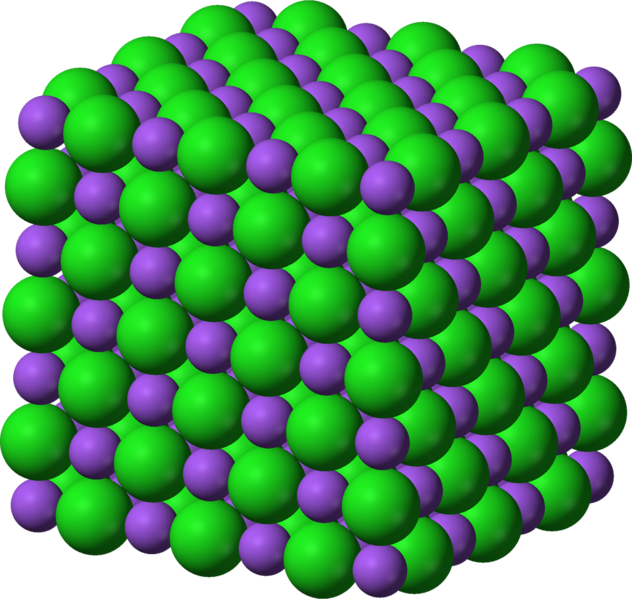
\includegraphics[width=0.5\textwidth]{photos/sodiumchloride_wikipedia.png}\\
\begin{caption}{A space filling model of the sodium chloride lattice}\end{caption}
 \end{center}

\end{minipage}
      \label{m38684*uid71}
            \subsection*{Properties of Ionic Compounds}
            \nopagebreak \noindent
        \label{m38684*id142811}Ionic compounds have a number of properties:\par 
        \label{m38684*id142815}\begin{itemize}[noitemsep]
            \label{m38684*uid72}\item Ions are arranged in a lattice structure
\label{m38684*uid73}\item Ionic solids are crystalline at room temperature
\label{m38684*uid74}\item The ionic bond is a strong electrostatic attraction. This means that ionic compounds are often hard and have high melting and boiling points
\label{m38684*uid75}\item Ionic compounds are brittle and bonds are broken along planes when the compound is stressed
\label{m38684*uid76}\item Solid crystals do not conduct electricity, but ionic solutions do
\end{itemize}
\label{m38684*secfhsst!!!underscore!!!id522}
            \begin{exercises}{Ionic compounds
        }
            \nopagebreak \noindent
        \label{m38684*id142562}\begin{enumerate}[noitemsep, label=\textbf{\arabic*}. ] 
%Question 1
            \label{m38684*uid57}\item Explain the difference between a \textsl{covalent} and an \textsl{ionic} bond.\newline
%Question 2
\label{m38684*uid58}\item Magnesium and chlorine react to form magnesium chloride.
\label{m38684*id142602}\begin{enumerate}[noitemsep, label=\textbf{\alph*}. ] 
            \label{m38684*uid59}\item What is the difference in electronegativity between these two elements?
\label{m38684*uid60}\item Give the chemical formula for:
\label{m38684*id142630}\begin{enumerate}[noitemsep, label=\textbf{\roman*}. ] 
            \label{m38684*uid61}\item a magnesium ion
\label{m38684*uid62}\item a chloride ion
\label{m38684*uid63}\item the ionic compound that is produced during this reaction
\end{enumerate}
        \label{m38684*uid64}\item Write a balanced chemical equation for the reaction that takes place.
\end{enumerate}
%Question 3
        \label{m38684*uid65}\item Draw Lewis diagrams to represent the following ionic compounds:
\label{m38684*id142697}\begin{enumerate}[noitemsep, label=\textbf{\alph*}. ] 
            \label{m38684*uid66}\item sodium iodide ($\text{NaI}$)
\label{m38684*uid67}\item calcium bromide ($\text{CaBr}{}_{2}$)
\label{m38684*uid68}\item potassium chloride ($\text{KCl}$)
\end{enumerate}
        \end{enumerate}
      \label{m38684*uid69}
\par \raisebox{-5 pt}{
\includegraphics[width=0.5cm]{col11305.imgs/summary_www.png}} Find the answers with the shortcodes:
 \par \begin{tabular}[h]{cccccc}
 (1.) lOq  &  (2.) lOl  &  (3.) lOi  & \end{tabular}
\end{exercises}

  \label{m38684**end}
         \section{Metallic Bonding}
    \nopagebreak
%            \label{m38694} $ \hspace{-5pt}\begin{array}{cccccccccccc}   
\includegraphics[width=0.75cm]{col11305.imgs/summary_video.png} &   \end{array} $ \hspace{2 pt}\raisebox{-5 pt}{} {(section shortcode: P10033 )} \par 
      \label{m38694*uid77}
            \subsection*{The nature of the metallic bond}
            \nopagebreak
        \label{m38694*id142901}The structure of a metallic bond is quite different from covalent and ionic bonds. In a metal bond, the valence electrons are \textsl{delocalised}, meaning that an atom's electrons do not stay around that one nucleus. In a metallic bond, the positive atomic nuclei (sometimes called the 'atomic kernels') are surrounded by a sea of delocalised electrons which are attracted to the nuclei (see figure below).\par 
\label{m38694*fhsst!!!underscore!!!id582}
\Definition{ \label{id2431026} Metallic bond} { \label{m38694*meaningfhsst!!!underscore!!!id582}
Metallic bonding is the electrostatic attraction between the positively charged atomic nuclei of metal atoms and the delocalised electrons in the metal.}
\begin{minipage}{.5\textwidth}
    \setcounter{subfigure}{0}
% \begin{figure}[h]
\begin{center}
\scalebox{0.8}{
\begin{pspicture}(-3,-3)(3,3)
\psframe(0,0)(5,5)
%row 1
\multirput(1,1)(1,0){4}{
\pscircle(0,0){.2}
\uput[r]{0}(-0.3,0){$+$}}
%row 2
\pscircle(1,2){.2}
\uput[r]{0}(0.7,2){$+$}
\pscircle(2,2){.2}
\uput[r]{0}(1.7,2){$+$}
\pscircle(3,2){.2}
\uput[r]{0}(2.7,2){$+$}
\pscircle(4,2){.2}
\uput[r]{0}(3.7,2){$+$}
%row 3
\pscircle(1,3){.2}
\uput[r]{0}(0.7,3){$+$}
\pscircle(2,3){.2}
\uput[r]{0}(1.7,3){$+$}
\pscircle(3,3){.2}
\uput[r]{0}(2.7,3){$+$}
\pscircle(4,3){.2}
\uput[r]{0}(3.7,3){$+$}
%row 4
\pscircle(1,4){.2}
\uput[r]{0}(0.7,4){$+$}
\pscircle(2,4){.2}
\uput[r]{0}(1.7,4){$+$}
\pscircle(3,4){.2}
\uput[r]{0}(2.7,4){$+$}
\pscircle(4,4){.2}
\uput[r]{0}(3.7,4){$+$}
%the electrons
\qdisk(0.2,0.5){1.5pt}
\qdisk(4.7,4.6){1.5pt}
\qdisk(1,4.5){1.5pt}
\qdisk(1.4,3.3){1.5pt}
\qdisk(2.8,1.7){1.5pt}
\qdisk(3.4,3){1.5pt}
\qdisk(4.3,3.2){1.5pt}
\qdisk(4.8,0.3){1.5pt}
\qdisk(2.5,2.5){1.5pt}
\qdisk(0.4,0.3){1.5pt}
\qdisk(1,0.6){1.5pt}
\qdisk(1.4,4.7){1.5pt}
\qdisk(0.6,2.1){1.5pt}
\qdisk(2.1,0.4){1.5pt}
\qdisk(3.4,0.7){1.5pt}
\qdisk(3,0.2){1.5pt}
\qdisk(4.5,0.4){1.5pt}
\qdisk(1.5,1.5){1.5pt}
\qdisk(0.3,3.7){1.5pt}
\qdisk(2.5,3.5){1.5pt}
\qdisk(4.7,1.5){1.5pt}
\qdisk(2.5,4.3){1.5pt}
\qdisk(3.2,4.4){1.5pt}
\qdisk(3.9,4.5){1.5pt}
\end{pspicture}
}
\end{center}
\begin{caption}{Positive atomic nuclei (+) surrounded by delocalised electrons ($\bullet$)}\end{caption}
\label{fig:an:metallic bond}
% \end{figure}      
\end{minipage}
\begin{minipage}{.5\textwidth}
 \begin{center}
  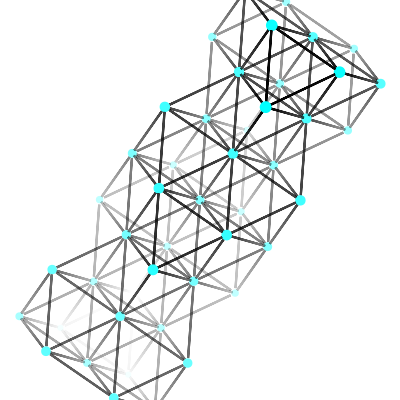
\includegraphics[width=0.6\textwidth]{photos/copper_structure.png}\\
\begin{caption}{Ball and stick model of copper}\end{caption}
 \end{center}

\end{minipage}
\subsection*{Properties of metals}
\begin{itemize}[noitemsep]
 \item Metals are \textsl{shiny}.
\item Metals \textsl{conduct electricity} because electrons are free to move.
\item Metals \textsl{conduct heat} because the positive nuclei are packed closely together and can easily transfer the heat.
\item Metals have a \textsl{high melting point} because the bonds are strong and a \textsl{high density} because of the tight packing of the nuclei.
\end{itemize}

        \label{m38694*id754}
            \begin{activity}{Building models}
            \nopagebreak
\begin{minipage}{.5\textwidth}
        \label{m38694*id87434}Using coloured balls (or jellytots) and sticks (or toothpicks) build models of each type of bonding. Think about how to represent each kind of bonding. For example, covalent bonding could be represented by simply connecting the balls with sticks to represent the molecules, while for ionic bonding you may wish to construct part of the crystal lattice. Do some research on types of crystal lattices (although the section on ionic bonding only showed the crystal lattice for sodium chloride, many other types of lattices exist) and try to build some of these. Share your findings with your class and compare notes to see what types of crystal lattices they found. How would you show metallic bonding?\par 
\end{minipage}
\begin{minipage}{.5\textwidth}
\scalebox{.6} % Change this value to rescale the drawing.
{
\begin{pspicture}(0,-4.44)(9.26,4.44)
\definecolor{color381b}{rgb}{0.8823529411764706,0.8823529411764706,0.8823529411764706}
\definecolor{color457b}{rgb}{0.7254901960784313,0.7254901960784313,0.7254901960784313}
\definecolor{color877}{rgb}{0.3137254901960784,0.3137254901960784,0.3137254901960784}
\definecolor{color878}{rgb}{0.47058823529411764,0.47058823529411764,0.47058823529411764}
\pspolygon[linewidth=0.04,fillstyle=solid,fillcolor=color381b](3.13,3.29)(4.11,4.25)(4.11,1.31)(3.13,0.33)
\pspolygon[linewidth=0.04,fillstyle=solid,fillcolor=color381b](0.17,3.31)(1.15,4.27)(1.15,1.33)(0.17,0.35)
\psframe[linewidth=0.04,dimen=outer,fillstyle=solid,fillcolor=color457b](4.13,4.31)(1.13,1.31)
\psframe[linewidth=0.04,dimen=outer](3.15,3.33)(0.15,0.33)
\psline[linewidth=0.04cm](3.13,3.31)(4.07,4.27)
\psdots[dotsize=0.3](1.15,1.35)
\psdots[dotsize=0.3](0.17,3.27)
\psdots[dotsize=0.3](1.13,4.25)
\psdots[dotsize=0.3](3.09,3.29)
\psdots[dotsize=0.3](4.07,4.27)
\psdots[dotsize=0.3](4.05,1.33)
\psdots[dotsize=0.3](0.17,0.37)
\psdots[dotsize=0.3](3.13,0.35)
\pspolygon[linewidth=0.04,fillstyle=solid,fillcolor=color381b](8.15,3.27)(9.13,4.23)(9.13,1.29)(8.15,0.31)
\pspolygon[linewidth=0.04,fillstyle=solid,fillcolor=color381b](5.19,3.29)(6.17,4.25)(6.17,1.31)(5.19,0.33)
\psframe[linewidth=0.04,dimen=outer,fillstyle=solid,fillcolor=color457b](9.15,4.29)(6.15,1.29)
\psframe[linewidth=0.04,dimen=outer](8.17,3.31)(5.17,0.31)
\psline[linewidth=0.04cm](8.15,3.29)(9.09,4.25)
\psdots[dotsize=0.3](6.17,1.33)
\psdots[dotsize=0.3](5.19,3.25)
\psdots[dotsize=0.3](6.15,4.23)
\psdots[dotsize=0.3](8.11,3.27)
\psdots[dotsize=0.3](9.09,4.25)
\psdots[dotsize=0.3](9.07,1.31)
\psdots[dotsize=0.3](5.21,0.33)
\pspolygon[linewidth=0.04,fillstyle=solid,fillcolor=color381b](5.13,-1.33)(6.11,-0.37)(6.11,-3.31)(5.13,-4.29)
\pspolygon[linewidth=0.04,fillstyle=solid,fillcolor=color381b](2.17,-1.31)(3.15,-0.35)(3.15,-3.29)(2.17,-4.27)
\psframe[linewidth=0.04,dimen=outer,fillstyle=solid,fillcolor=color457b](6.13,-0.31)(3.13,-3.31)
\psframe[linewidth=0.04,dimen=outer](5.15,-1.29)(2.15,-4.29)
\psline[linewidth=0.04cm](5.13,-1.31)(6.07,-0.35)
\psdots[dotsize=0.3](3.15,-3.27)
\psdots[dotsize=0.3](2.17,-1.35)
\psdots[dotsize=0.3](3.13,-0.37)
\psdots[dotsize=0.3](5.09,-1.33)
\psdots[dotsize=0.3](6.07,-0.35)
\psdots[dotsize=0.3](6.05,-3.29)
\psdots[dotsize=0.3](2.17,-4.25)
\psdots[dotsize=0.3](5.13,-4.27)
\psdots[dotsize=0.3](7.13,2.39)
\psdots[dotsize=0.3](8.17,0.33)
\psdots[dotsize=0.3,linecolor=color877](4.39,-1.97)
\psdots[dotsize=0.3,linecolor=color878](2.63,-2.27)
\psdots[dotsize=0.3,linecolor=color878](5.61,-2.17)
\psdots[dotsize=0.3](4.13,-0.81)
\psdots[dotsize=0.3](3.97,-3.81)
\psdots[dotsize=0.3](3.85,-2.47)
\end{pspicture} 
}
\end{minipage}
\end{activity}
\label{m38694*eip-515}
    \setcounter{subfigure}{0}
	\begin{figure}[H] % horizontal\label{m38694*bonds-1}
    \textnormal{Khan academy video on bonding - 1} \nopagebreak
  \label{m38694*yt-media1}\label{m38694*yt-video1}
            \raisebox{-5 pt}{ 
\includegraphics[width=0.5cm]{col11305.imgs/summary_www.png}} { (Video:  P10034 )}
 \end{figure}       \par \label{m38694*secfhsst!!!underscore!!!id617}
            \begin{exercises}{Bonding
        }
            \nopagebreak \noindent
        \label{m38694*id143111}\begin{enumerate}[noitemsep, label=\textbf{\arabic*}. ] 
%Question 1 
           \label{m38694*uid86}\item Give two examples of everyday objects that contain:
\label{m38694*id143127}\begin{enumerate}[noitemsep, label=\textbf{\alph*}. ] 
            \label{m38694*uid87}\item covalent bonds
\label{m38694*uid88}\item ionic bonds
\label{m38694*uid89}\item metallic bonds
\end{enumerate}
%Question 2 
               \label{m38694*uid90}\item Complete the table which compares the different types of bonding:
    % \textbf{m38694*id143180}\par
          \begin{table}[H]
    % \begin{table}[H]
    % \\ 'id2900564' '1'
        \begin{center}
      \label{m38694*id143180}
    \noindent
      \begin{tabular}{|l|l|l|l|}\hline
         &
        \textbf{Covalent} &
        \textbf{Ionic} &
        \textbf{Metallic} \\ \hline
        Types of atoms involved &
         &
         &
        \\ \hline
        Nature of bond between atoms &
         &
         &
       \\ \hline
        Melting point (high/low) &
         &
         &
       \\ \hline
        Conducts electricity? (yes/no) &
         &
         &
      \\ \hline
        Other properties &
         &
         &
       \\ \hline
    \end{tabular}
      \end{center}
\end{table}
    \par
%Question 3
          \label{m38694*uid91}\item Complete the table below by identifying the type of bond (covalent, ionic or metallic) in each of the compounds:
    % \textbf{m38694*id143418}\par
          \begin{table}[H]
    % \begin{table}[H]
    % \\ 'id2900649' '1'
        \begin{center}
      \label{m38694*id143418}
    \noindent
      \begin{tabular}{|l|l|}\hline
        \textbf{Molecular formula} &
        \textbf{Type of bond} \\ \hline
        $\text{H}_{2}\text{SO}_{4}$ &
        \\ \hline
        $\text{FeS}$ &
        \\ \hline
        $\text{NaI}$ &
         \\ \hline
        $\text{MgCl}_{2}$ &
        \\ \hline
        $\text{Zn}$ &
       \\ \hline
    \end{tabular}
      \end{center}
\end{table}
    \par
%Question 4 in book, 3 on FM
          \label{m38694*uid92}\item Which of these substances will conduct electricity most effectively? Give a reason for your answer.\newline
%Question 5
\label{m38694*uid93}\item Use your knowledge of the different types of bonding to explain the following statements:
\label{m38694*id143618}\begin{enumerate}[noitemsep, label=\textbf{\alph*}. ] 
            \label{m38694*uid94}\item A sodium chloride crystal does not conduct electricity.
\label{m38694*uid95}\item Most jewellery items are made from metals.
\label{m38694*uid96}\item It is very hard to break a diamond.
\item Pots are made from metals, but their handles are made from plastic.
\end{enumerate}
                \end{enumerate}
  \label{m38694**end}
\par \raisebox{-5 pt}{
\includegraphics[width=0.5cm]{col11305.imgs/summary_www.png}} Find the answers with the shortcodes:
 \par \begin{tabular}[h]{cccccc}
 (1.) l3h  &  (2.) l3u  &  (3.) l3J  &  (4.) l3J  &  (5.) ljj  & \end{tabular}
\end{exercises}
         \section{Writing formulae}
    \nopagebreak
%            \label{m38689} $ \hspace{-5pt}\begin{array}{cccccccccccc}   
\includegraphics[width=0.75cm]{col11305.imgs/summary_fullmarks.png} &   
\includegraphics[width=0.75cm]{col11305.imgs/summary_video.png} &   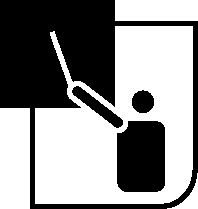
\includegraphics[width=0.75cm]{col11305.imgs/summary_presentation.png} &   \end{array} $ \hspace{2 pt}\raisebox{-5 pt}{} {(section shortcode: P10035 )} \par 
In chapter~\ref{chap:classification} you learnt about the writing of chemical formulae. Table~\ref{tab:ions} shows some of the common anions and cations that you should know.
    % \textbf{m38689*uid99}\par
          \begin{table}[H]
    % \begin{table}[H]
    % \\ '' '0'
        \begin{center}
      \label{m38689*uid99}
    \noindent
      \begin{tabular}{|l|l|l|l|}\hline
                  \textbf{Name of compound ion} &
                  \textbf{formula} &  \textbf{Name of compound ion} & \textbf{formula} \\ \hline
        Carbonate & $\mathrm{CO}_{3}^{2-}$ & Nitrite & $\mathrm{NO}_{2}^{-}$ \\ \hline
        Sulphate &  $\mathrm{SO}_{4}^{2-}$ & Hydrogen sulphite & $\mathrm{HSO}_{3}^{-}$ \\ \hline
        Hydroxide & ${\mathrm{OH}}^{-}$ & Hydrogen sulphate & $\mathrm{HSO}_{4}^{-}$ \\ \hline
        Ammonium & $\mathrm{NH}_{4}^{+}$ & Dihydrogen phosphate & ${\mathrm{H}}_{2}\mathrm{PO}_{4}^{-}$ \\ \hline
        Nitrate & $\mathrm{NO}_{3}^{-}$ & Hypochlorite & ${\mathrm{ClO}}^{-}$ \\ \hline
        Hydrogen carbonate & $\mathrm{HCO}_{3}^{-}$ & Acetate (ethanoate) & ${\mathrm{CH}}_{3}{\mathrm{COO}}^{-}$ \\ \hline
        Phosphate & $\mathrm{PO}_{4}^{3-}$ & Oxalate & ${\mathrm{C}}_{2}\mathrm{O}_{4}^{2-}$ \\ \hline
        Chlorate & $\mathrm{ClO}_{3}^{-}$ &  Oxide & ${\mathrm{O}}^{2-}$ \\ \hline
        Cyanide & ${\mathrm{CN}}^{-}$ & Peroxide & $\mathrm{O}_{2}^{2-}$ \\ \hline
        Chromate & $\mathrm{CrO}_{4}^{2-}$ & Sulphide & ${\mathrm{S}}^{2-}$ \\ \hline
        Permanganate & $\mathrm{MnO}_{4}^{-}$ & Sulphite & $\mathrm{SO}_{3}^{2-}$ \\ \hline
        Thiosulphate & ${\mathrm{S}}_{2}\mathrm{O}_{3}^{2-}$ & Manganate & $\mathrm{MnO}_{4}^{2-}$ \\ \hline
        Phosphide & ${\mathrm{P}}^{3-}$ & Hydrogen phosphate & $\mathrm{HPO}_{4}^{3-}$ \\ \hline
    \end{tabular}
      \end{center}
    \caption{Table showing common compound ions and their formulae}
\label{tab:ions}
\end{table}
    \par
	\par

            \subsection*{Chemical compounds: names and masses}
            \nopagebreak
\label{m38689*uid97124}In chapter~\ref{chap:atom} you learnt about atomic masses. In this chapter we have learnt that atoms can combine to form compounds. Molecules are formed when atoms combine through covalent bonding, for example ammonia is a molecule made up of three hydrogen atoms and one nitrogen atom. The \textbf{relative molecular mass} ($\text{M}$) of ammonia ($\text{NH}_{3}$) is: \\
\begin{eqnarray*}
 \text{M} & = & \text{relative atomic mass of one nitrogen} + \text{relative atomic mass of three hydrogens} \\
 & = & 14,0 + 3(1,01)  \\ 
 & = & 17,03
\end{eqnarray*}
One molecule of $\text{NH}_{3}$ will have a  mass of $17,03\text{ units}$. When sodium reacts with chlorine to form sodium chloride, we do not get a molecule of sodium chloride, but rather a sodium chloride crystal lattice. Remember that in ionic bonding molecules are not formed. We can also calculate the mass of one unit of such a crystal. We call this a \textbf{formula unit} and the mass is called the \textbf{formula mass}. The formula mass for sodium chloride is:
 \begin{eqnarray*}
 \text{M} & = & \text{relative atomic mass of one sodium atom} + \text{relative atomic mass of one chlorine atom}\\
 & = & 23,0 + 35,45 \\
 & = & 58,45
\end{eqnarray*} 
The formula mass for $\text{NaCl}$ is $58,45~\text{units}$.
      \label{m38689*secfhsst!!!underscore!!!id822}
            \begin{exercises}{Chemical formulae
        }
            \nopagebreak
        \label{m38689*id145052}\begin{enumerate}[noitemsep, label=\textbf{\arabic*}. ] 
%Question 1
            \label{m38689*uid100}\item 
Complete the following table. The cations at the top combine with the anions on the left. The first row is done for you. Also include the names of the compounds formed and the anions.
          \begin{table}[H]
        \begin{center}
      \label{m38689*id145067}
    \noindent
      \begin{tabular}{|p{1cm}|p{1.5cm}|p{2cm}|p{2cm}|p{2cm}|p{2cm}|}\hline
        &\textbf{ $\text{Na}^{+}$} & \textbf{$\text{Mg}^{2+}$} & \textbf{$\text{Al}^{3+}$} & \textbf{$\text{NH}_{4}^{+}$} & \textbf{$\text{H}^{+}$} \\ \hline
\multirow{2}{1cm}{\textbf{$\text{Br}^{-}$ name:}} & $\text{NaBr}$  & $\text{MgBr}_2$  & $\text{AlBr}_3$  & $(\text{NH}_{4})\text{Br}$  & $\mathrm{HBr}$  \\ 
 & sodium bromide & magnesium bromide & aluminium bromide & ammonium bromide & hydrogen bromide \\ \hline
\textbf{$\text{S}^{2-}$ name:} & & & & & \\ \hline
\textbf{$\text{P}^{3-}$ name:} & & & & & \\ \hline
\textbf{$\text{MnO}_{4}^{-}$ name:} & & & & & \\ \hline
\textbf{$\text{Cr}_{2}\text{O}_{7}^{2-}$ name:} & & & & & \\ \hline
\textbf{$\text{HPO}_{4}^{2-}$ name:} & & & & & \\ \hline
    \end{tabular}
      \end{center}
\end{table}
    \par
%Question 2
          \label{m38689*uid101}\item Write the chemical formulae for each of the following compounds:
\label{m38689*id145444}\begin{enumerate}[noitemsep, label=\textbf{\alph*}. ] 
            \label{m38689*uid102}\item hydrogen cyanide
\label{m38689*uid103}\item carbon dioxide
\label{m38689*uid104}\item sodium carbonate
\label{m38689*uid105}\item ammonium hydroxide
\label{m38689*uid106}\item barium sulphate
\item copper (II) nitrate
\end{enumerate}
Calculate the relative molecular mass or formula mass for each of the compounds above.
                \end{enumerate}
\label{m38689*cid121}
\par \raisebox{-5 pt}{
\includegraphics[width=0.5cm]{col11305.imgs/summary_www.png}} Find the answers with the shortcodes:
 \par \begin{tabular}[h]{cccccc}
 (1.) ljD  &  (2.) ljW  & \end{tabular}
\end{exercises}
    \label{m38689*eip-891}
    \setcounter{subfigure}{0}
	\begin{figure}[H] % horizontal\label{m38689*slidesharefigure}
    \label{m38689*slidesharemedia}\label{m38689*slideshareflash}\raisebox{-5 pt}{ 
\includegraphics[width=0.5cm]{col11305.imgs/summary_www.png}} { (Presentation:  P10036 )}
 \end{figure}       \par \label{m38689*cid13}
            \section{Summary}
            \nopagebreak
      \label{m38689*id147386}\begin{itemize}[noitemsep]
            \label{m38689*uid136}\item A \textbf{chemical bond} is the electrostatic attraction between positive nuclei and negative electrons to combine atoms to form new substances.
\label{m38689*uid137}\item Atoms are more \textbf{reactive}, and therefore more likely to bond, when their outer electron orbitals are not full. Atoms are less reactive when these outer orbitals contain the maximum number of electrons. This explains why the noble gases do not react.
\label{m38689*uid142}\item When atoms bond, electrons are either shared or exchanged.
\label{m38689*uid143}\item \textbf{Covalent bonding} occurs between the atoms of non-metals and involves a sharing of electrons so that the orbitals of the outermost energy levels in the atoms are filled.
\label{m38689*uid145}\item A \textbf{double} or \textbf{triple bond} occurs if there are two or three electron pairs that are shared between the same two atoms.
\label{m38689*uid147}\item \textbf{Lewis} notation is one way of representing molecular structure. In Lewis notation, dots and crosses are used to represent the valence electrons around the central atom.
\label{m38689*uid150}\item An \textbf{ionic bond} occurs between atoms where there is a large difference in electronegativity. An exchange of electrons takes place and the atoms are held together by the electrostatic force of attraction between the resulting oppositely-charged ions.
\label{m38689*uid151}\item Ionic solids are arranged in a \textbf{crystal lattice} structure.
\label{m38689*uid152}\item Ionic compounds have a number of specific \textbf{properties}, including their high melting and boiling points, brittle nature, the lattice structure of solids and the ability of ionic solutions to conduct electricity.
\label{m38689*uid153}\item A \textbf{metallic bond} is the electrostatic attraction between the positively charged nuclei of metal atoms and the delocalised electrons in the metal.
\label{m38689*uid154}\item Metals also have a number of properties, including their ability to conduct heat and electricity, their metallic lustre (shine), the fact that they are both malleable (flexible) and ductile (stretchable) and their high melting point and density.
\label{m38689*uid155}\item The valence electrons of atoms and the way they bond, can be used to determine the \textbf{chemical formulae} of compounds.
\end{itemize}
\label{m38689*secfhsst!!!underscore!!!id1181}
            \begin{eocexercises}{Chemical Bonding}
            \nopagebreak \noindent
      \label{m38689*id147820}\begin{enumerate}[noitemsep, label=\textbf{\arabic*}. ] 
%Question 1
            \label{m38689*uid158}\item Explain the meaning of each of the following terms
\label{m38689*id147842}\begin{enumerate}[noitemsep, label=\textbf{\alph*}. ] 
            \label{m38689*uid159}\item ionic bond
\label{m38689*uid160}\item covalent bond
\end{enumerate}
%Question 2
                \label{m38689*uid162}\item Which ONE of the following best describes the bond formed between carbon and hydrogen?
\label{m38689*id147923}\begin{enumerate}[noitemsep, label=\textbf{\alph*}. ] 
            \label{m38689*uid163}\item metallic bond
\label{m38689*uid164}\item covalent bond
\label{m38689*uid165}\item ionic bond
\end{enumerate}
%Question 3 
               \label{m38689*uid171}\item Which of the following reactions will \textsl{not} take place? Explain your answer.
\label{m38689*id148047}\begin{enumerate}[noitemsep, label=\textbf{\alph*}. ] 
            \label{m38689*uid172}\item $\mathrm{H}+\mathrm{H}\to {\mathrm{H}}_{2}$\label{m38689*uid173}\item $\mathrm{Ne}+\mathrm{Ne}\to {\mathrm{Ne}}_{2}$\label{m38689*uid174}\item $\mathrm{Cl}+\mathrm{Cl}\to {\mathrm{Cl}}_{2}$\end{enumerate}
%Question 4
                \label{m38689*uid175}\item Draw the Lewis structure for each of the following:
\label{m38689*id148172}\begin{enumerate}[noitemsep, label=\textbf{\alph*}. ] 
            \label{m38689*uid176}\item calcium
\label{m38689*uid177}\item iodine
\label{m38689*uid178}\item hydrogen bromide ($\text{HBr}$)
\label{m38689*uid179}\item nitrogen dioxide ($\text{NO}{}_{2}$)
\end{enumerate}
%Question 5
                \label{m38689*uid180}\item Given the following Lewis structure, where X and Y each represent a different element...
    \setcounter{subfigure}{0}
	\begin{figure}[H] % horizontal\label{m38689*id148255}
\begin{center}
\begin{pspicture}(-2,-0.8)(3,0.6)
%\psgrid[gridcolor=gray]
\rput(-0.3,0){\Large \textbf{X}}
\rput(0.6,0){\Large \textbf{Y}}
\rput(1.5,0){\Large \textbf{X}}
\rput(0.6,-0.9){\Large \textbf{X}}

\rput{90}(0.6,0){\uput{9pt}[d](0,0){$\times$ $\bullet$}}
\rput{270}(0.6,0){\uput{9pt}[d](0,0){$\times$ $\bullet$}}
\uput{9pt}[u](0.6,0){$\times$ $\times$}
\uput{9pt}[d](0.6,0){$\times$ $\bullet$}
\end{pspicture}
\end{center}
 \end{figure}      

 \label{m38689*id148261}\begin{enumerate}[noitemsep, label=\textbf{\alph*}. ] 
            \label{m38689*uid181}\item What is the valency of $\mathrm{X}$?
\label{m38689*uid182}\item What is the valency of $\mathrm{Y}$?
\label{m38689*uid183}\item Which elements could $\mathrm{X}$ and $\mathrm{Y}$ represent?
\end{enumerate}
%Question 6
\item Complete the following table:
\begin{table}[H]
\begin{center}
 \begin{tabular}{|l|l|l|l|} \hline
  & \textbf{$\text{K}^{+}$} & \textbf{$\text{Ca}^{2+}$} & \textbf{$\text{NH}_{4}^{+}$} \\ \hline
\textbf{$\text{OH}^{-}$} & & & \\ \hline   
\textbf{$\text{O}^{2-}$} & & & \\ \hline   
\textbf{$\text{NO}_{3}^{-}$} & & & \\ \hline   
\textbf{$\text{PO}_{4}^{3-}$} & & & \\ \hline   
 \end{tabular}
\end{center}
\end{table}
%Question 7
              \label{m38689*uid185}\item Potassium dichromate is dissolved in water.
\label{m38689*id148361}\begin{enumerate}[noitemsep, label=\textbf{\alph*}. ] 
            \label{m38689*uid186}\item Give the name and chemical formula for each of the ions in solution.
\label{m38689*uid187}\item What is the chemical formula for potassium dichromate?
\end{enumerate}
                \end{enumerate}
  \label{m38689**end}
  \label{6cd7661dc7a31822d94f8eef4ac8e3a5**end}
\par \raisebox{-5 pt}{
\includegraphics[width=0.5cm]{col11305.imgs/summary_www.png}} Find the answers with the shortcodes:
 \par \begin{tabular}[h]{cccccc}
 (1.) ljZ  &  (2.) ljB  &  (3.) l36  &  (4.) l3H  &  (5.) l3s  &  (6.) ljk  &  (7.) ljK  & \end{tabular}
\end{eocexercises}
